% The structure ((1, 2), 3, 4) viewed as a tree, for Section 2.2.2.
%
% Upstream's figure labels the root and the one interior node with Lisp's
% printed form. Ours uses the tuple notation the section is written in, which
% is the whole reason this figure is redrawn rather than inherited: the shape
% of the tree is the same in both languages, but the labels are not.
%
% Leaves are spaced evenly and every parent sits at the midpoint of its
% children, matching the layout of the other tree figures in the book.

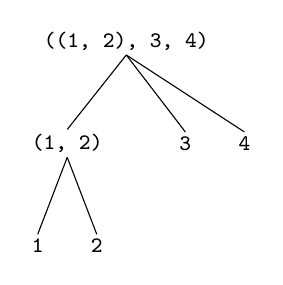
\begin{tikzpicture}[
  x = 15mm, y = -13mm,
  every node/.style = {font=\ttfamily\footnotesize, inner sep=1.5pt},
  edge/.style = {draw, thin},
]

\node (root) at (1.0, 0) {((1, 2), 3, 4)};
\node (sub)  at (0.5, 1) {(1, 2)};
\node (n3)   at (1.5, 1) {3};
\node (n4)   at (2.0, 1) {4};
\node (n1)   at (0.25, 2) {1};
\node (n2)   at (0.75, 2) {2};

% Anchored at the base of the parent rather than its border: the root's label
% is wide enough that border-to-border edges would leave from under the middle
% of the text instead of from the node.
\foreach \parent/\child in {root/sub, root/n3, root/n4, sub/n1, sub/n2}
  \draw[edge] (\parent.south) -- (\child.north);

\end{tikzpicture}
